\section{Revisão da Literatura/Considerações Gerais}


\subsection{O que são jogos?}

\begin{frame}

    \frametitle{O que é um jogo?}

    \begin{figure}[!htbp]
    	\centering
    	%\caption{Exemplo de figura (caption é opcional)}
    	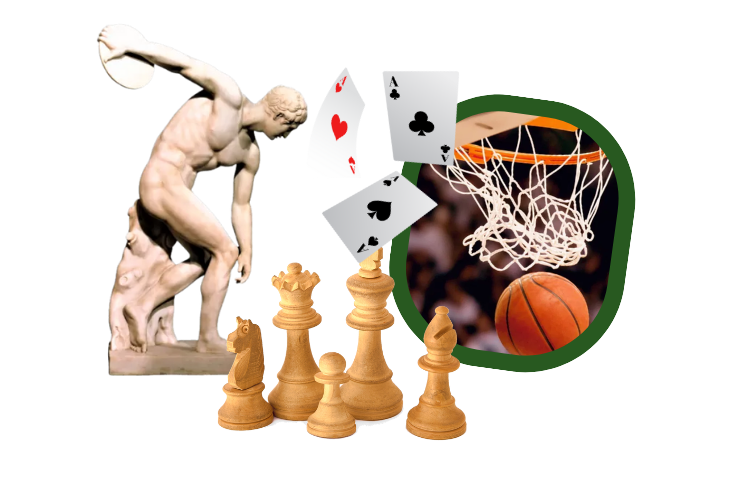
\includegraphics[scale=0.5]{imagens/JogosTradicionais.png}
    	%\\\small{\textbf{Fonte:} Elaborada pelo autor (fonte é opcional)}%
    \end{figure}

\end{frame}

\begin{frame}
	
	\frametitle{Mas e um jogo Eletrônico?}
	
	\begin{block}{Definição de Crawford}
		“Um jogo é um sistema fechado e formal que representa subjetivamente um subconjunto da realidade.”
	\end{block}
	
	\begin{itemize} 
	\textbf{Um jogo eletrônico é:}
		\item \textbf{Sistema fechado:} O jogo é um produto completo e independente em sua estrutura;
		\item \textbf{Representação Subjetiva:} Uma simulação de uma parte da realidade (ou fantasia) focada na experiência do jogador.
	\end{itemize}
	
\end{frame}


\begin{frame}

    \frametitle{O que é um jogo eletrônico?}

     \begin{figure}[!htbp]
    	\centering
    	%\caption{Exemplo de figura (caption é opcional)}
    	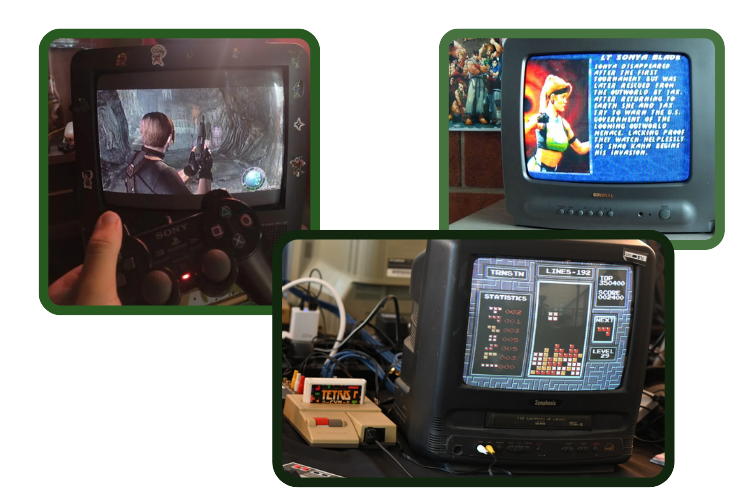
\includegraphics[scale=0.53]{imagens/JogosEletronicos.png}
    	%\\\small{\textbf{Fonte:} Elaborada pelo autor (fonte é opcional)}%
    \end{figure}

\end{frame}


\subsection{Gêneros de jogos}

\begin{frame}

    \frametitle{Gênero de ação}

    Subgêneros dos jogos de ação: FPS, Luta, Plataforma
    
    \begin{figure}[!htbp]
    	\centering
    	%\caption{Exemplo de figura (caption é opcional)}
    	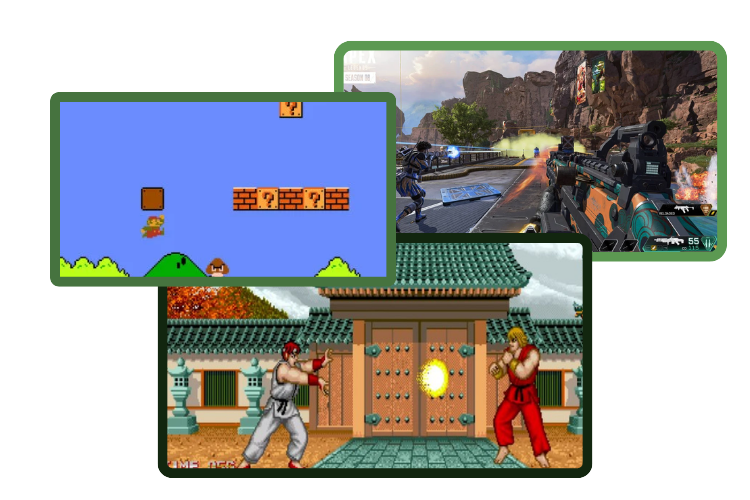
\includegraphics[scale=0.5]{imagens/JogosAção.png}
    	%\\\small{\textbf{Fonte:} Elaborada pelo autor (fonte é opcional)}%
    \end{figure}
    
    

\end{frame}


\begin{frame}

    \frametitle{Gênero de Puzzle}

    \begin{figure}[!htbp]
    	\centering
    	%\caption{Exemplo de figura (caption é opcional)}
    	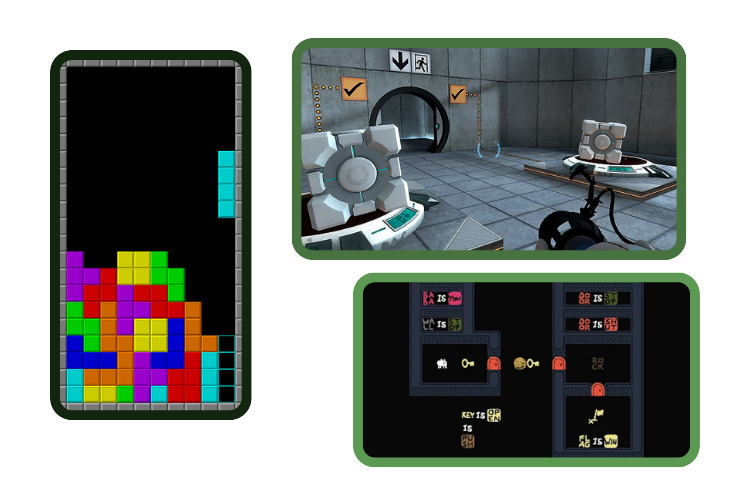
\includegraphics[scale=0.5]{imagens/JogosQuebraCabeça.png}
    	%\\\small{\textbf{Fonte:} Elaborada pelo autor (fonte é opcional)}%
    \end{figure}

\end{frame}

\begin{frame}
	
	\frametitle{Gêneros}
	
	Existem muitos gêneros e subgênero de jogos, como por exemplo: Simulação, Aventura, RPG, Estratégia, SoulsLike, etc.
	
	\begin{figure}[!htbp]
		\centering
		%\caption{Exemplo de figura (caption é opcional)}
		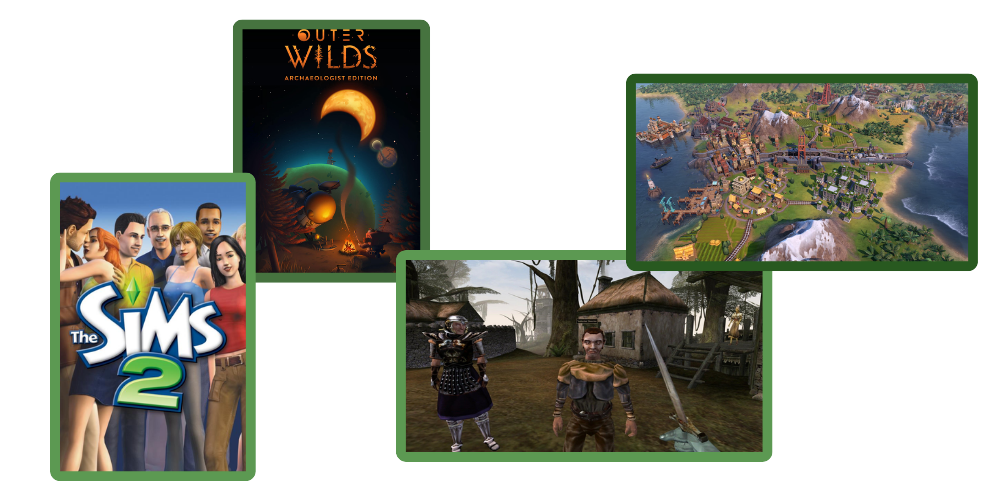
\includegraphics[scale=0.4]{imagens/JogosGeneros (2).png}
		%\\\small{\textbf{Fonte:} Elaborada pelo autor (fonte é opcional)}%
	\end{figure}
	
\end{frame}

\subsection{Tecnologia para desenvolvimento de jogos}

\begin{frame}

    \frametitle{Motores gráficos}
	
	Para desenvolver um jogo, é necessário conhecimentos de várias áreas distintas como: música, programação de algoritmos, desenhos, gráficos e outros.
	\\
	Um motor gráficos são ambientes para desenvolvimento de jogos que abstrai esses conhecimentos, gerencia \textit{loops} e possui módulos para criação de diferentes tipos de jogos.
    
     \begin{figure}[!htbp]
     	\centering
     	\caption{Ciclo de vida de um jogo}
     	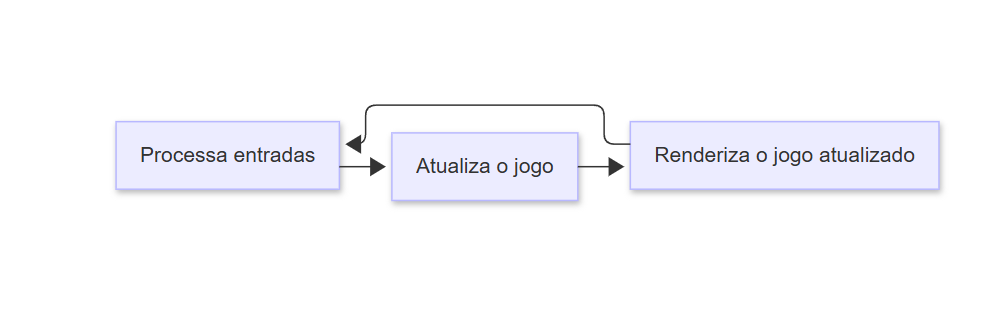
\includegraphics[scale=0.42]{imagens/LoopEngineJogo.png}
     	%\\\small{\textbf{Fonte:} Elaborada pelo autor (fonte é opcional)}%
     \end{figure}

\end{frame}


\begin{frame}

    \frametitle{Godot Engine}
    
    \begin{figure}[!htbp]
    	\centering
    	
\includegraphics[scale=0.05]{imagens/Godot_icon.png}
    	%\\\small{\textbf{Fonte:} Elaborada pelo autor (fonte é opcional)}%
    \end{figure}

    \begin{itemize}
    	\item Criação de jogos 2D e 3D;
    	\item Baseado em nós (nodes): Gráficos, física, interface e outros;
    	\item Scripts em GDScripts;
    \end{itemize}

\end{frame}

\begin{frame}
	
	\frametitle{Java/LibGDX}
	
	 \begin{columns}[t]
		
		\begin{column}{7cm}
			

			 \begin{itemize}
				\item Linguagem baseada no paradigma de orientação a objeto;
				\item Encapsular dados e criar métodos;
				\item Manipulação de dados;
			\end{itemize}
			
			
			\begin{figure}[!htbp]
				\centering
				
\includegraphics[scale=0.1]{imagens/java-coffee-cup-logo.png}
				%\\\small{\textbf{Fonte:} Elaborada pelo autor (fonte é opcional)}%
			\end{figure}
			
		\end{column}
		
		\begin{column}{7cm}
			
			\begin{itemize}
				\item Framework de java, usa a OpenGL;
				\item Jogos 2D e 3D;
				\item Módulos para criação de jogos;
				\item Manipulaçao de bitmaps e editor de texturas;
			\end{itemize}
			
			\begin{figure}[!htbp]
				\centering
				
\includegraphics[scale=0.05]{imagens/LibGDXlogo.png}
				%\\\small{\textbf{Fonte:} Elaborada pelo autor (fonte é opcional)}%
			\end{figure}
			
		\end{column}
		
	\end{columns}
	
	
	
\end{frame}

\begin{frame}
	
	\frametitle{C++/Raylib}
	
	\begin{columns}[t]
		
		\begin{column}{7cm}
			
			\begin{itemize}
				\item Abstrair dados;
				\item Suportar paradigmas da orientação objeto e procedural;
				\item Alto nível, a partir da linguagem de programação C;
				\item Maior flexibilidade na hora de escolher o paradigma;
			\end{itemize}
			
			\begin{figure}[!htbp]
				\centering
				
\includegraphics[scale=0.02]{imagens/ISO_C++_Logo.png}
				%\\\small{\textbf{Fonte:} Elaborada pelo autor (fonte é opcional)}%
			\end{figure}
			
		\end{column}
		
		\begin{column}{7cm}
			
			\begin{itemize}
				\item Biblioteca de programação de jogos 2D e 3D;
				\item Não há uma documentação;
				\item Uma lista com funções disponíveis;
				\item Suporte para PC (Desktop e Web) e celulares;
			\end{itemize}
			
			\begin{figure}[!htbp]
				\centering
				
\includegraphics[scale=0.2]{imagens/Raylib_logo.png}
				%\\\small{\textbf{Fonte:} Elaborada pelo autor (fonte é opcional)}%
			\end{figure}
			
		\end{column}
		
	\end{columns}
	
	
\end{frame}

\begin{frame}
	
	\frametitle{Python/Pygame}
	
	\begin{columns}[t]
		
		\begin{column}{7cm}
			
			\begin{itemize}
				\item Identação importante e sintaxe simples;
				\item Módulos de lista, dicionários e outros;
				\item Adicionar bibliotecas de terceiros;
				\item Multi-paradigma;
			\end{itemize}
			
			\begin{figure}[!htbp]
				\centering
				
\includegraphics[scale=0.02]{imagens/Python-logo-notext.png}
				%\\\small{\textbf{Fonte:} Elaborada pelo autor (fonte é opcional)}%
			\end{figure}
			
		\end{column}
		
		\begin{column}{7cm}
			
			\begin{itemize}
				\item Framework para Python;
				\item Feita sobre a biblioteca SDL;
				\item Deixar mais acessível para criação de jogos;
				\item Módulos para construir um jogo;
			\end{itemize}
			
			\begin{figure}[!htbp]
				\centering
				
\includegraphics[scale=0.2]{imagens/pygame_logo.png}
				%\\\small{\textbf{Fonte:} Elaborada pelo autor (fonte é opcional)}%
			\end{figure}
			
		\end{column}
		
	\end{columns}
	
	
\end{frame}
